% Soubory musí být v kódování, které je nastaveno v příkazu \usepackage[...]{inputenc}

\documentclass[%        Základní nastavení
%  draft,    				  % Testovací překlad
  12pt,       				% Velikost základního písma je 12 bodů
  a4paper,    				% Formát papíru je A4
  oneside,      			% Jednostranný tisk
	%twoside,      			% Dvoustranný tisk (kapitoly a další důležité části tedy začínají na lichých stranách)
	unicode,						% Záložky a metainformace ve výsledném  PDF budou v kódování unicode
]{report}				    	% Dokument třídy 'zpráva', vhodná pro sazbu závěrečných prací s kapitolami

\usepackage[utf8]		  %	Kódování zdrojových souborů je UTF-8
	{inputenc}					% Balíček pro nastavení kódování zdrojových souborů

\usepackage[				% Nastavení geometrie stránky
	bindingoffset=10mm,		% Hřbet pro vazbu
	hmargin={25mm,25mm},	% Vnitřní a vnější okraj  (jsou nehezky shodné; jakási úroveň estetiky je dosažena pomocí hřbetu)
	vmargin={25mm,34mm},	% Horní a dolní okraj
	footskip=17mm,			  % Velikost zápatí
	nohead,					      % Bez záhlaví
	marginparsep=2mm,		  % Vzdálenost marginálií
	marginparwidth=18mm,	% Šířka marginálií
]{geometry}

\usepackage{sectsty}
	%přetypuje nadpisy všech úrovní na bezpatkové, kromě \chapter, která je přenastavena zvlášť v thesis.sty
	\allsectionsfont{\sffamily}

\usepackage{graphicx} % Balíček 'graphicx' pro vkládání obrázků
											% Nutné pro vložení logotypů školy a fakulty

\usepackage[          % Balíček 'acronym' pro sazby zkratek a symbolů
	nohyperlinks				% Nebudou tvořeny hypertextové odkazy do seznamu zkratek
]{acronym}						
											% Nutné pro použití prostředí 'acronym' balíčku 'thesis'

\usepackage[
	breaklinks=true,		% Hypertextové odkazy mohou obsahovat zalomení řádku
	hypertexnames=false % Názvy hypertext. odkazů budou tvořeny nezávisle na názvech TeXu
]{hyperref}						% Balíček 'hyperref' pro sazbu hypertextových odkazů
											% Nutné pro použití příkazu 'pdfsettings' balíčku 'thesis'

\usepackage{pdfpages} % Balíček umožňující vkládat stránky z PDF souborů
                      % Nutné při vkládání titulních listů a zadání přímo
                      % ve formátu PDF z informačního systému

\usepackage{enumitem} % Balíček pro nastavení mezerování v odrážkách
  \setlist{topsep=0pt,partopsep=0pt,noitemsep} % konkrétní nastavení

\usepackage{cmap} 		% Balíček cmap zajišťuje, že PDF vytvořené `pdflatexem' je
											% plně "prohledávatelné" a "kopírovatelné"

%\usepackage{upgreek}	% Balíček pro sazbu stojatých řeckých písmem
											%% např. stojaté pí: \uppi
											%% např. stojaté mí: \upmu (použitelné třeba v mikrometrech)
											%% pozor, grafická nekompatibilita s fonty typu Computer Modern!
                      
%\usepackage{amsmath} %balíček pro sabu náročnější matematiky                 

\usepackage{dirtree}	% sazba adresářové struktury
                      % vhodné pro prezentaci obsahu elektronické přílohy (např. CD)

\usepackage[formats]{listings}	% Balíček pro sazbu zdrojových textů
\lstset{              % nastavení
%	Definice jazyka použitého ve výpisech
%    language=[LaTeX]{TeX},	% LaTeX
%	language={Matlab},		% Matlab
	language={C},           % jazyk C
    basicstyle=\ttfamily,	% definice základního stylu písma
    tabsize=2,			% definice velikosti tabulátoru
    inputencoding=utf8,         % pro soubory uložené v kódování UTF-8
		columns=fixed,  %fixed nebo flexible,
		fontadjust=true %licovani sloupcu
    extendedchars=true,
    literate=%  definice symbolů s diakritikou
    {á}{{\'a}}1
    {č}{{\v{c}}}1
    {ď}{{\v{d}}}1
    {é}{{\'e}}1
    {ě}{{\v{e}}}1
    {í}{{\'i}}1
    {ň}{{\v{n}}}1
    {ó}{{\'o}}1
    {ř}{{\v{r}}}1
    {š}{{\v{s}}}1
    {ť}{{\v{t}}}1
    {ú}{{\'u}}1
    {ů}{{\r{u}}}1
    {ý}{{\'y}}1
    {ž}{{\v{z}}}1
    {Á}{{\'A}}1
    {Č}{{\v{C}}}1
    {Ď}{{\v{D}}}1
    {É}{{\'E}}1
    {Ě}{{\v{E}}}1
    {Í}{{\'I}}1
    {Ň}{{\v{N}}}1
    {Ó}{{\'O}}1
    {Ř}{{\v{R}}}1
    {Š}{{\v{S}}}1
    {Ť}{{\v{T}}}1
    {Ú}{{\'U}}1
    {Ů}{{\r{U}}}1
    {Ý}{{\'Y}}1
    {Ž}{{\v{Z}}}1
}

%%%%%vlastni balicky
\usepackage{makecell}
\usepackage{siunitx}
\sisetup{output-decimal-marker = {,}}
\DeclareSIUnit\LSB{LSB}
\usepackage{subfigure}
\usepackage{tablefootnote}
\usepackage{amsmath}



%%%%%%%%%%%%%%%%%%%%%%%%%%%%%%%%%%%%%%%%%%%%%%%%%%%%%%%%%%%%%%%%%
%%%%%%      Definice informací o dokumentu             %%%%%%%%%%
%%%%%%%%%%%%%%%%%%%%%%%%%%%%%%%%%%%%%%%%%%%%%%%%%%%%%%%%%%%%%%%%%

% V tomto souboru se nastavují téměř veškeré informace, proměnné mezi studenty:
% jméno, název práce, pohlaví atd.
% Tento soubor je SDÍLENÝ mezi textem práce a prezentací k obhajobě -- netřeba něco nastavovat na dvou místech.

\usepackage[
%%% Z následujících voleb jazyka lze použít pouze jednu
  czech-english,		% originální jazyk je čeština, překlad je anglicky (výchozí)
  %english-czech,	% originální jazyk je angličtina, překlad je česky
  %slovak-english,	% originální jazyk je slovenština, překlad je anglicky
  %english-slovak,	% originální jazyk je angličtina, překlad je slovensky
%
%%% Z následujících voleb typu práce lze použít pouze jednu
  semestral,		  % semestrální práce (výchozí)
  %bachelor,			%	bakalářská práce
  %master,			  % diplomová práce
  %treatise,			% pojednání o disertační práci
  %doctoral,			% disertační práce
%
%%% Z následujících voleb zarovnání objektů lze použít pouze jednu
%  left,				  % rovnice a popisky plovoucích objektů budou zarovnány vlevo
	center,			    % rovnice a popisky plovoucích objektů budou zarovnány na střed (vychozi)
%
]{thesis}   % Balíček pro sazbu studentských prací


%%% Jméno a příjmení autora ve tvaru
%  [tituly před jménem]{Křestní}{Příjmení}[tituly za jménem]
% Pokud osoba nemá titul před/za jménem, smažte celý řetězec '[...]'
\author{Marek}{Coufal}

%%% Identifikační číslo autora (VUT ID)
\butid{240598}

%%% Pohlaví autora/autorky
% (nepoužije se ve variantě english-czech ani english-slovak)
% Číselná hodnota: 1...žena, 0...muž
\gender{0}

%%% Jméno a příjmení vedoucího/školitele včetně titulů
%  [tituly před jménem]{Křestní}{Příjmení}[tituly za jménem]
% Pokud osoba nemá titul před/za jménem, smažte celý řetězec '[...]'
\advisor[Ing.]{Jan}{Král}[Ph.D.]

%%% Jméno a příjmení oponenta včetně titulů
%  [tituly před jménem]{Křestní}{Příjmení}[tituly za jménem]
% Pokud osoba nemá titul před/za jménem, smažte celý řetězec '[...]'
% Nastavení oponenta se uplatní pouze v prezentaci k obhajobě;
% v případě, že nechcete, aby se na titulním snímku prezentace zobrazoval oponent, pouze příkaz zakomentujte;
% u obhajoby semestrální práce se oponent nezobrazuje (jelikož neexistuje)
% U dizertační práce jsou typicky dva až tři oponenti. Pokud je chcete mít na titulním slajdu, prosím ručně odkomentujte a upravte jejich jména v definici "VUT title page" v souboru thesis.sty.
\opponent[doc.\ Mgr.]{Křestní}{Příjmení}[Ph.D.]

%%% Název práce
%  Parametr ve složených závorkách {} je název v originálním jazyce,
%  parametr v hranatých závorkách [] je překlad (podle toho jaký je originální jazyk).
%  V případě, že název Vaší práce je dlouhý a nevleze se celý do zápatí prezentace, použijte příkaz
%  \def\insertshorttitle{Zkác.\ náz.\ práce}
%  kde jako parametr vyplníte zkrácený název. Pokud nechcete zkracovat název, budete muset předefinovat,
%  jak se vytváří patička slidu. Viz odkaz: https://bit.ly/3EJTp5A
\title[Indoor Positioning Based on Inercial Measurement Unit
]{Měření polohy uvnitř budov pomocí inerciální jednotky
}

%%% Označení oboru studia
%  Parametr ve složených závorkách {} je název oboru v originálním jazyce,
%  parametr v hranatých závorkách [] je překlad
\specialization[Electronics and Communication Technologies]{Elektronika a komunikační technologie}

%%% Označení ústavu
%  Parametr ve složených závorkách {} je název ústavu v originálním jazyce,
%  parametr v hranatých závorkách [] je překlad
%\department[Department of Control and Instrumentation]{Ústav automatizace a měřicí techniky}
%\department[Department of Biomedical Engineering]{Ústav biomedicínského inženýrství}
%\department[Department of Electrical Power Engineering]{Ústav elektroenergetiky}
%\department[Department of Electrical and Electronic Technology]{Ústav elektrotechnologie}
%\department[Department of Physics]{Ústav fyziky}
%\department[Department of Foreign Languages]{Ústav jazyků}
%\department[Department of Mathematics]{Ústav matematiky}
%\department[Department of Microelectronics]{Ústav mikroelektroniky}
\department[Department of Radio Electronics]{Ústav radioelektroniky}
%\department[Department of Theoretical and Experimental Electrical Engineering]{Ústav teoretické a experimentální elektrotechniky}
%\department[Department of Telecommunications]{Ústav telekomunikací}
%\department[Department of Power Electrical and Electronic Engineering]{Ústav výkonové elektrotechniky a elektroniky}

%%% Označení fakulty
%  Parametr ve složených závorkách {} je název fakulty v originálním jazyce,
%  parametr v hranatých závorkách [] je překlad
%\faculty[Faculty of Architecture]{Fakulta architektury}
\faculty[Faculty of Electrical Engineering and~Communication]{Fakulta elektrotechniky a~komunikačních technologií}
%\faculty[Faculty of Chemistry]{Fakulta chemická}
%\faculty[Faculty of Information Technology]{Fakulta informačních technologií}
%\faculty[Faculty of Business and Management]{Fakulta podnikatelská}
%\faculty[Faculty of Civil Engineering]{Fakulta stavební}
%\faculty[Faculty of Mechanical Engineering]{Fakulta strojního inženýrství}
%\faculty[Faculty of Fine Arts]{Fakulta výtvarných umění}
%
%Nastavení logotypu (v hranatych zavorkach zkracene logo, ve slozenych plne):
\facultylogo[logo/FEKT_zkratka_barevne_PANTONE_CZ]{logo/VUT_barevne_PANTONE_CZ}

%%% Rok odevzdání práce
\graduateyear{2024}
%%% Akademický rok odevzdání práce
\academicyear{2023/24}

%%% Datum obhajoby (uplatní se pouze v prezentaci k obhajobě)
\date{5.\,1.\,2023} 

%%% Místo obhajoby
% Na titulních stránkách bude automaticky vysázeno VELKÝMI písmeny (pokud tyto stránky sází šablona)
\city{Brno}

%%% Abstrakt
\abstract[%
Překlad abstraktu
(v~angličtině, pokud je originálním jazykem čeština či slovenština; v~češtině či slovenštině, pokud je originálním jazykem angličtina)
]{%
Abstrakt práce v~originálním jazyce
}

%%% Klíčová slova
\keywrds[%
Překlad klíčových slov
(v~angličtině, pokud je originálním jazykem čeština či slovenština; v~češtině či slovenštině, pokud je originálním jazykem angličtina)
]{%
Klíčová slova v~originálním jazyce
}

%%% Poděkování
\acknowledgement{%
Rád bych poděkoval vedoucímu bakalářské/diplomové/disertační práce
panu Ing.~XXX YYY, Ph.D.\ za odborné vedení,
konzultace, trpělivost a~podnětné návrhy k~práci.
}%  % do tohoto souboru doplňte údaje o sobě, druhu práce, názvu...

%%%%%%%%%%%%%%%%%%%%%%%%%%%%%%%%%%%%%%%%%%%%%%%%%%%%%%%%%%%%%%%%%%%%%%%%

%%%%%%%%%%%%%%%%%%%%%%%%%%%%%%%%%%%%%%%%%%%%%%%%%%%%%%%%%%%%%%%%%%%%%%%%
%%%%%%     Nastavení polí ve Vlastnostech dokumentu PDF      %%%%%%%%%%%
%%%%%%%%%%%%%%%%%%%%%%%%%%%%%%%%%%%%%%%%%%%%%%%%%%%%%%%%%%%%%%%%%%%%%%%%
%% Při načteném balíčku 'hyperref' lze použít příkaz '\pdfsettings':
\pdfsettings
%  Nastavení polí je možné provést také ručně příkazem:
%\hypersetup{
%  pdftitle={Název studentské práce},    	% Pole 'Document Title'
%  pdfauthor={Autor studenstké práce},   	% Pole 'Author'
%  pdfsubject={Typ práce}, 						  	% Pole 'Subject'
%  pdfkeywords={Klíčová slova}           	% Pole 'Keywords'
%}
%%%%%%%%%%%%%%%%%%%%%%%%%%%%%%%%%%%%%%%%%%%%%%%%%%%%%%%%%%%%%%%%%%%%%%%

\pdfmapfile{=vafle.map}

%%%%%%%%%%%%%%%%%%%%%%%%%%%%%%%%%%%%%%%%%%%%%%%%%%%%%%%%%%%%%%%%%%%%%%%
%%%%%%%%%%%       Začátek dokumentu               %%%%%%%%%%%%%%%%%%%%%
%%%%%%%%%%%%%%%%%%%%%%%%%%%%%%%%%%%%%%%%%%%%%%%%%%%%%%%%%%%%%%%%%%%%%%%
\begin{document}
\pagestyle{empty} %vypnutí číslování stránek

%%% Vložení desek -- od září 2021 na žádost fakulty nepoužíváno
%\includepdf[pages=1]%  buďto generovaných informačním systémem
  %{pdf/student-desky}% název souboru nesmí obsahovat mezery!
%%% NEBO vytvoření desek z balíčku
%%\makecover
%%%
%\oddpage % při dvojstranném tisku přidá prázdnou stránku
%% kazdopádně ale:
%\setcounter{page}{1} %resetovaní čítače stránek -- desky do číslování nezahrnujeme

%% Vložení titulního listu
\includepdf[pages=1]%    buďto generovaného informačním systémem
  {pdf/student-titulka}% název souboru nesmí obsahovat mezery!
%% NEBO vytvoření titulní stránky z balíčku
%\maketitle
%%
\oddpage  % při dvojstranném tisku se přidá prázdná stránka
   
%% Vložení zadání
\includepdf[pages=1]%   buďto generovaného informačním systémem
  {pdf/student-zadani}% název souboru nesmí obsahovat mezery!
%% NEBO lze vytvořit prázdný list příkazem ze šablony
%\patternpage{}%
%	{\sffamily\Huge\centering ZDE VLOŽIT LIST ZADÁNÍ}%
%	{\sffamily\centering Z~důvodu správného číslování stránek}
%%
\oddpage% při dvojstranném tisku se přidá prázdná stránka

%% Vysázení stránky s abstraktem
\makeabstract

% Vysázení stránky s rozšířeným abstraktem
% (pokud píšete práci v češtině či slovenštině, vložení rozšířeného abstraktu zrušte;
%  pro semestrální projekt také není potřeba rozšířený abstrakt uvádět)
% Vysázení stránky s rozšířeným abstraktem
% (týká se pouze bc. a dp. prací psaných v angličtině, viz Směrnice rektora 72/2017)
\cleardoublepage
\noindent
{\large\sffamily\bfseries\MakeUppercase{Rozšířený abstrakt}}
\\
Výtah ze směrnice rektora 72/2017:\\
\emph{Bakalářská a diplomová práce předložená v angličtině musí obsahovat rozšířený abstrakt v češtině
nebo slovenštině (čl. 15). To se netýká studentů, kteří studují studijní program akreditovaný v
angličtině.}
(čl. 3, par. 7)\\
\emph{Nebude-li vnitřní normou stanoveno jinak, doporučuje se rozšířený abstrakt o rozsahu přibližně 3
normostrany, který bude obsahovat úvod, popis řešení a shrnutí a zhodnocení výsledků.}
(čl. 15, par. 5)

%%% Vysázení citace práce
\makecitation

%%% Vysázení prohlášení o samostatnosti
\makedeclaration

%%% Vysázení poděkování
\makeacknowledgement

%%% Vysázení obsahu
\tableofcontents

%%% Vysázení seznamu obrázků
% (vynechejte, pokud máte dva nebo méně obrázků)
\listoffigures

%%% Vysázení seznamu tabulek
% (vynechejte, pokud máte dvě nebo méně tabulek)
\listoftables

%%% Vysázení seznamu výpisů kódu
% (vynechejte, pokud máte dva nebo méně výpisů)
\lstlistoflistings

\cleardoublepage\pagestyle{plain}   % zapnutí číslování stránek

%Pro vkládání kapitol i příloh používejte raději \include než \input
%%% Vložení souboru 'text/uvod.tex' s úvodem
\chapter*{Úvod}
\phantomsection
\addcontentsline{toc}{chapter}{Úvod}

Tato práce se zabývá poměrně komplexní problematikou inerciální navigace pro použití uvnitř budov a jejím sestrojením, tedy určováním polohy pomocí „black boxu“ který své údaje o pohybu určí primárně z údajů o lineárním zrychlení z akcelerometru a úhlové rychlosti z gyroskopu pro omezení potřeby neustálé dostupnosti signálu z globálních navigačních systémů.

Jsou popsány algoritmy pro zpracování dat šestiosé inerciální jednotky s nehybně umístěnými \ac{MEMS} gyroskopy a akcelerometry, což umožňuje značnou miniaturizaci a snížení ceny, v porovnání s osvědčenými systémy využívající velké a složité mechanické konstrukce gimbalů a gyroskopů. Přestože se přesnost senzorů stále zlepšuje, i díky malé odchylce měřených dat může rychle narůstat chyba odhadované polohy díky integraci úhlové rychlosti a dvojité integraci lineárního zrychlení. Z tohoto důvodu je jednotka opatřena i magnetometrem a \ac{GNSS} modulem pro možnost fúze dalších dat pro co největší zmenšení chyby, tomuto se ovšem bude věnovat až navazující bakalářská práce.

Jsou také věnovány kapitoly samotnému návrhu inerciální jednotky, minimálním požadavkům na komunikace a jejich počtům a rychlostem, způsobu zaznamenávání dat a celkovému blokovému konceptu. V poslední kapitole je také popsán návrh desky plošných spojů inerciální jednotky. 

%%% Vložení souboru 'text/cile.tex' s úvodem
\chapter*{Cíle práce}
\phantomsection
\addcontentsline{toc}{chapter}{Cíle práce}

Konkrétní specifikace cílů, které má autor v~práci vyřešit.
Tato kapitola je \emph{volitelná} -- pokud váš studijní program nevyžaduje zvláštní kapitolu s cíli,
cíle specifikujte v~rámci Úvodu.

%%% Vložení souboru 'text/reseni' s popisem řešení práce
% (rozdělte na více souborů či kapitol, pokud je vhodné)
\chapter{Teoretická část studentské práce}
\section{Porovnání navigačních systémů}



%%% Vložení souboru 'text/vysledky' s popisem vysledků práce
% (rozdělte na více souborů či kapitol, pokud je vhodné)
\chapter{Výsledky studentské práce}
\section{Hardware inerciální jednotky}

\begin{figure}[h]
    \centering
    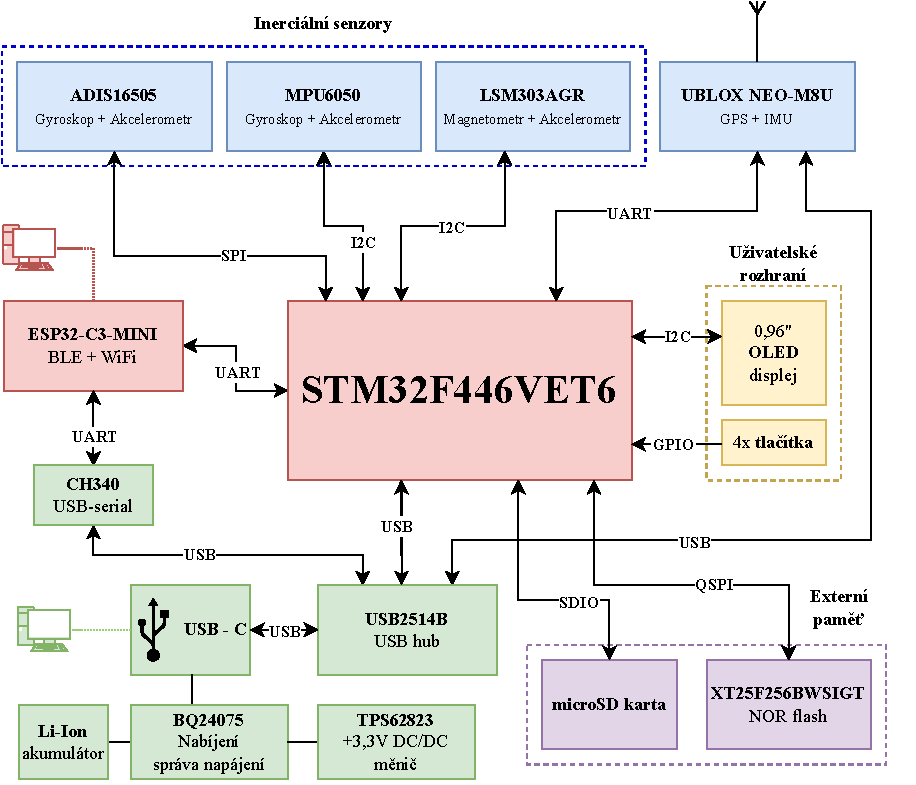
\includegraphics[width=\textwidth]{obrazky/IMUnav_H00_block}
    \caption{Blokové schéma inerciální jednotky}
\end{figure}

Hardware inerciální jednotky je realizován tak, aby umožňoval zaznamenávat hodnoty změřené inerciálními senzory a poskytovat dohromady data o rozměru 9~DoF (akcelerometr, gyroskop a magnetometr). Jednotka také obsahuje GPS modul s vestavěným IMU, jehož použití by mohlo být vhodné například v prostorech s alespoň částečným pokrytím signálu GPS.

Naměřená data je možné uložit do externí NOR Flash paměti připojené k MCU, popřípadě lze využít i kartu typu microSD. K přenosu dat pro jejich následné zpracování v PC primárně slouží ESP32-C3, umožňující bezdrátovou komunikaci přes Wifi, nebo Bluetooth. Konektor USB typu C umožňuje nabíjení vestavěného Li-Ion akumulátoru jednotky a komunikaci mezi PC a ESP32, GPS modulem a hlavním MCU skrze vestavěný USB rozbočovač. Toto rozhraní je plánované pro použití např. ke konfiguračním, nebo ladícím účelům.

Pro jednoduchou volnost pohybu je jednotka napájena jedním Li-Ion akumulátorem velikosti 18650, při záznamu dat tedy nebude potřeba externího zdroje energie. Grafický OLED displej a 4 tlačítka slouží jako uživatelské rozhraní při používání jednotky.

\subsection{Akcelerometr a gyroskop} \label{AccGyroText}
Jednotka obsahuje dvě 6~DoF IMU (gyroskop s akcelerometrem) rozdílných parametrů a řádově rozdílné ceny. Takto odlišné součástky byly vybrány proto, aby bylo možné porovnat vliv přesnosti, šumu a driftu senzorů na následně zpracovaná data.
V Tabulce \ref{table:fyzikalniPorovnaniIMU} jsou porovnány důležité parametry senzorů MPU6050 a ADIS16505-2. Pro účely inerciální navigace je důležitý zejména nízký drift senzorů, aby při integraci dat k vyhodnocení polohy nebyla integrována i driftová chyba, což má za výsledek velmi nepřesné zpracování hodnot.

\begin{table}[h!]
\centering
\begin{tabular}{c||c c c}
\hline 
Model IMU & MPU6050 & ADIS16505-2 & jednotka \\ 
\hline
\hline 
\multicolumn{4}{c}{Parametry gyroskopů} \\
\hline
\hline
Dynamický rozsah  & \makecell{programovatelný, \\ $\pm 250$, $\pm 500$, \\$\pm 1000$, $\pm 2000$} & $\pm 500$ & $\SI[per-mode = symbol]{}{\degree\per\second}$ \\ 
\hline 
Citlivost  \tablefootnote{Pro porovnání citlivosti byl vybrán dynamický rozsah $\SI[per-mode = symbol]{500}{\degree\per\second}$ senzoru MPU6050 pro možnost porovnání hodnoty s druhým senzorem} & $65,5$ & $2621440$ & $\SI[per-mode = symbol]{}{\LSB\per(\degree\per\second)}$ \\ 
\hline 
Drift v ose x a z & $\pm 20$ & $\pm 0,14$ & $\SI[per-mode = symbol]{}{\degree\per\second}$ \\ 
\hline 
Drift v ose y & $\pm 20$ & $\pm 1,4$ & $\SI[per-mode = symbol]{}{\degree\per\second}$ \\ 
\hline 
\makecell{Efektivní hodnota hustoty \\šumu při 10Hz pro osy x a y} & 0,005 & 0,0043 & $\SI{}{\degree\per\second\per\sqrt{\Hz}}$ \\ 
\hline 
\makecell{Efektivní hodnota hustoty \\šumu při 10Hz pro osu z} & 0,005 & 0,0034 & $\SI{}{\degree\per\second\per\sqrt{\Hz}}$ \\ 
\hline 
\hline 
\multicolumn{4}{c}{Parametry akcelerometrů} \\
\hline
\hline
Dynamický rozsah  & \makecell{programovatelný, \\ $\pm 19,6$, $\pm 39,2$, \\$\pm 78,4$, $\pm 156,8$} & $\pm 78,4$ & $\SI[per-mode = symbol]{}{\metre\per\second\squared}$ \\ 
\hline 
Citlivost  \tablefootnote{Pro porovnání citlivosti byl vybrán dynamický rozsah $\SI[per-mode = symbol]{78,4}{\metre\per\second\squared}$ senzoru MPU6050 pro možnost porovnání hodnoty s druhým senzorem} & $418$ & $26756268$ & $\SI[per-mode = symbol]{}{\LSB\per(\metre\per\second\squared)}$ \\ 
\hline 
Drift v ose x a y & $\pm 0,491$ & $\pm 0,0196$ & $\SI[per-mode = symbol]{}{\metre\per\second\squared}$ \\ 
\hline 
Drift v ose z & $\pm 0,785$ & $\pm 0,0196$ & $\SI[per-mode = symbol]{}{\metre\per\second\squared}$ \\ 
\hline 
\makecell{Efektivní hodnota hustoty \\šumu při 10Hz pro osy x a y} & 3924 & 167 & $\SI{}{\micro\metre\per\second\squared\per\sqrt{\Hz}}$ \\ 
\hline 
\makecell{Efektivní hodnota hustoty \\šumu při 10Hz pro osu z} & 3924 & 243 & $\SI{}{\micro\metre\per\second\squared\per\sqrt{\Hz}}$ \\ 
\hline 

\end{tabular} 
\caption{Porovnání základních parametrů gyroskopů \cite{euxR3Yh5ol4JWNAi} \cite{UZFqHmQU7ZzI3OLB}} 
\label{table:fyzikalniPorovnaniIMU}
\end{table} 


Integrovaný obvod MPU6050 je standardní 6 osé MEMS IMU, vhodné mimo jiné pro použití v mobilních zařízeních a dalších podobných aplikacích. Jeho vnitřní gyroskop a akcelerometr má softwarově přepínatelné rozsahy měřených veličin. Kromě inerciálních senzorů má i vestavěný signálový procesor pro fúzi a filtrování dat přímo v integrovaném obvodu. Tato funkce může být vhodná pro odlehčení výpočetního výkonu hlavního procesoru, ovšem pro účely této práce nebude signálový procesor využit, jelikož se měřená data budou zpracovávat až po jejich naměření v PC, ne v reálném čase. Vzorkovací frekvence gyroskopu je 8 kHz a akcelerometru 1 kHz, oba senzory mají 16bitové rozlišení.
\cite{euxR3Yh5ol4JWNAi}

MPU6050 disponuje rozhraním I2C s maximální frekvencí hodinového signálu 400 kHz. \cite{euxR3Yh5ol4JWNAi}
Pokud bychom chtěli vyčítat ze senzoru data při maximální možné vzorkovací frekvenci, byla by potřeba minimální přenosová rychlost sběrnice:
$$ f_{\mathrm{clk}}=3~\mathrm{osy} \times(f_{\mathrm{gyro}} + f_{\mathrm{acc}})\times (\mathrm{16bitů} + 2 \times \mathrm{ACK})=3\times(8000+1000)\times(16+2)=\SI{486}{\kilo\hertz}$$
Při vyčítání dat o maximální vzorkovací frekvenci jsme omezeni samotným I2C rozhraním senzoru (využití maximální vzorkovací frekvence je teoreticky možné krátkodobě, pomocí interního 1kB FIFO zásobníku).\cite{euxR3Yh5ol4JWNAi}

Jelikož pro účely inerciální navigace stačí vzorkovací frekvence dat v  řádu stovek~Hz \cite{Wei2022}, tak není tato limitace omezující. Senzor je propojen s hlavním MCU přes I2C sběrnici s frekvencí hodinového signálu 400 kHz a není sdílena s žádným jiným zařízením, aby bylo možné, v případě potřeby, využít maximální dostupný potenciál senzoru (i přestože je reálná potřeba vzorkovací frekvence nižší).

Integrovaný obvod ADIS16505-2 je precizní 6 osé MEMS IMU, vhodné pro použití v průmyslových a navigačních aplikacích s poměrně nízkým driftem a vysokou přesností. Na rozdíl od MPU6050 nemá přepínatelný dynamický rozsah, je fixně daný variantou součástky. Vzorkovací frekvence gyroskopu i akcelerometru je 2 kHz, oba senzory mají 32bitové rozlišení. S hlavním MCU komunikuje přes sběrnici SPI s maximální frekvencí hodinového signálu 2,1 Mhz. \cite{UZFqHmQU7ZzI3OLB} Pokud budeme chtít vyčítat data ze senzoru při maximální možné vzorkovací frekvenci, bude potřeba minimální přenosová rychlost sběrnice: 
$$ f_{\mathrm{clk}}=3~\mathrm{osy} \times(f_{\mathrm{gyro}} + f_{\mathrm{acc}})\times \mathrm{32bitů}=3\times(2000+2000)\times 32=\SI{384}{\kilo\hertz}$$
Nejsme tedy omezeni maximální frekvencí hodinového signálu a můžeme teoreticky využívat senzor i při nejvyšší možné rychlosti.

Výrobce prodává tento obvod ve variantě 100 pinového BGA čipu, ale i jako vývojovou desku osazenou senzorem a kolíkovou lištou pro jednodušší práci s osazením DPS. \cite{UZFqHmQU7ZzI3OLB} Hardware jednotky byl navržen tak, aby bylo možné využít jak samotný BGA čip, tak i hotový modul s konektorem.

\subsection{Magnetometr}
Vzhledem k tomu, že výběr komerčně dostupných 9 DoF (akcelerometr, gyroskop a magnetometr) je značně omezený, popřípadě součástky prodávané jako 9osé IMU jsou ve skutečnosti moduly více součástek na jedné desce, tak je ve výsledném obvodovém zapojení použit senzor magnetické indukce jakožto samostatná součástka. 

Přestože fúze dat z magnetometru může mít pozitivní dopady na zmenšení chyby trajektorie \cite{Tkhorenko2018}, jeho použití uvnitř budov je značně omezené vzhledem k jednoduché ovlivnitelnosti měření blízkými feromagnetickými látkami, silovými rozvody elektřiny a pod. Proto nebyly na výběr magnetometru kladeny vysoké požadavky a slouží spíše pro porovnání vlivu přítomnosti / absence naměřených dat z tohoto senzoru.

K tomuto účelu byl vybrán běžně dostupný obvod LSM303AGR, který kromě magnetometru v pouzdře obsahuje i akcelerometr, ten ovšem nebude pro potřeby práce využit, jelikož tuto funkci obstarávají součástky z kapitoly \ref{AccGyroText}.

Magnetometr komunikuje s hlavním MCU přes sběrnici I2C s maximální vzorkovací frekvencí 150 Hz, dynamickým rozsahem $ \pm \SI{4.915}{\milli\tesla} $ a 16bitovým rozlišením. \cite{RD5DwZcremhT6bgp}

\subsection{GNSS}
Zajímavou a uživatelsky přívětivou kombinaci GNSS a inerciální navigace poskytuje například firma u-blox s řadou modulů podporující funkci „dead reckoning“. Jedná se o navigační moduly s vestavěným IMU, určené zejména do oblasti automotive. Jejich typický příklad použití, dle výrobce, je navigace aut, kdy při běžném provozu je zafixovaný signál z GNSS a při výpadku signálu (vjezd do garáže, tunelu apod.) je navigace modulem stále poskytována na základě dat z IMU. \cite{DLQg9bT6V1GWKhxh}

Navigační modul u-blox NEO-M8U byl vybrán a implementován do obvodového zapojení inerciální navigační jednotky.
Výrobce udává, že modul zvládne odhadovat polohu po ztrátě signálu GNSS po dobu 60 s s typickou odchylkou 10 \% trajektorie. Dále také modul při zapnutí odpovídající funkce umí využít interní IMU ke zvýšení maximální rychlosti aktualizace polohy až na 30 Hz. Jeho využití v rámci této práce může být různé, například pro navigaci v místech s alespoň částečným pokrytím signálu GNSS. \cite{DLQg9bT6V1GWKhxh}

NEO-M8U umí využívat všechny světové navigační systémy (uvedeny v tabulce~\ref{table:gnssBands})
\begin{table}[h!]
\caption{Podporované družicové systémy. \cite{DLQg9bT6V1GWKhxh} }
\centering
\begin{tabular}{c|c c }

GNSS systém & Pásmo & Frekvence (MHz) \\ 
\hline 
\hline
GPS & L1C/A & 1575,42 \\ 

GLONASS & L1OF & 1602 \\ 

BeiDou & B1 & 1561,098 \\ 

Galileo & E1-B/C & 1575,42 \\ 

\end{tabular} 

\label{table:gnssBands}
\end{table} 

Tento modul komunikuje s hlavním MCU přes sběrnici UART, pomocí standardizovaných NMEA příkazů v textové podobě, nebo pomocí binárního protokolu UBX, který je specifikován výrobcem. Použití protokolu NMEA je omezené pouze na standardní funkce GNSS modulů, pokud chceme využít speciálních funkcí, například inerciální navigace, je nutné použít proprietární protokol UBX. \cite{DLQg9bT6V1GWKhxh} NEO-M8U také disponuje USB portem, skrz který je možné modul ovládat a konfigurovat pomocí PC aplikace výrobce. Tento port je připojen na integrovaný USB rozbočovač a lze jej využít například pro vývojové účely.

\subsection{Paměť}
\begin{table}[h!]
\centering
\begin{tabular}{c|c}

Senzor & Odhadovaný bitrate \\ 
\hline 
\hline 
ADIS16505-2 & 375 kbit/s \\ 

MPU-6050 & 422 kbit/s \\ 

LSM303AGR & 7 kbit/s \\ 

NEO-M8U & 1 kbit/s \\ 
\hline

Celkem & 805 kbit/s (0,1MB/s) \\ 

\end{tabular} 
\caption{Odhad celkového bitratu pro záznam dat} 
\label{table:memoryBW}
\end{table} 
V případě, že bychom chtěli zaznamenávat data ze všech senzorů při jejich maximálních vzorkovacích frekvencích, nebude množství změřených dat zanedbatelné. V tabulce \ref{table:memoryBW} je hrubý odhad potřebné rychlosti záznamu dat pro tento krajní případ. Pokud bude měření trvat např. 2 minuty, vygenerujeme dohromady 12 MB dat, což převyšuje velikost paměti většiny dostupných MCU.

Z tohoto důvodu je v obvodovém zapojení inerciální jednotky implementována 32MB NOR Flash paměť, propojená s hlavním MCU přes sběrnici QUADSPI s maximální možnou hodinovou frekvencí 120 Mhz, měla by tedy být pro potřeby této aplikace dostačující. \cite{CgaRYSTpwKhEZZr7}

Kromě výše popsané Flash paměti jednotka obsahuje i slot na microSD kartu, která by z uživatelského hlediska mohla být jednodušší k použití, ovšem při zápisu může latence SD karty být (krátkodobě) až stovky ms \cite{Kraewinkel2020}. To by mohlo znemožnit její použití v případě, že by hlavní MCU měl nedostatek volné paměti RAM pro krátkodobé uchování dat, proto bude o její využití rozhodnuto až později.

\subsection{Uživatelské rozhraní}
\begin{figure}[h]
    \centering
    \includegraphics[width=0.3\textwidth]{obrazky/OLED}
    \caption{Fotografie grafického OLED displeje}
\end{figure}
Pro ovládání uživatelem disponuje jednotka grafickým OLED displejem s úhlopříčkou 0,96 palce a rozlišením $ 128 \times 64 $ pixelů, který je připojený přes sběrnici I2C. Společně s 4 tlačítky by měl poskytnout dostatečně univerzální a pohodlné uživatelské rozhraní.

\subsection{Napájení}
Inerciální jednotka je napájena z jednoho Li-Ion akumulátoru velikosti 18650. Nabíjení je realizováno obvodem BQ24075RGT, který monitoruje nabíjecí odebíraný proud jednotkou. Proud, kterým je nabíjen akumulátor je regulován tak, aby nepřekročil maximální hranici 900 mA z USB portu. \cite{F5eZCtr2LLRsr9NT}

Všechny součásti inerciální jednotky (až na RTC a zálohovací registry hlavního MCU a GPS modulu) jsou napájeny skrz DC/DC měnič z výstupního vývodu tohoto nabíjecího obvodu. V případě, že je připojena jednotka do USB a nabíjí se, na výstupním pinu nabíjecího obvodu je napájecí napětí USB portu. Díky tomu nedochází k velkým ztrátám pokud je jednotka zapnuta a nabíjí se zároveň. Jestliže je USB odpojeno, skrz interní tranzistor je jednotka napájena z akumulátoru. \cite{F5eZCtr2LLRsr9NT}

Nabíjecí obvod také umožňuje kompletní odpojení napájení jednotky přes jeden z vývodů. Toho je využito pro ochranu akumulátoru proti podvybití pomocí zapojení S/R klopného obvodu na napájení USB a jednoho z výstupů procesoru. Napětí akumulátoru je měřeno pomocí ADC mikrokontroléru. Jestliže klesne pod definovanou úroveň, pomocí pulzu bude celý obvod odpojen od napájení až do té doby, dokud uživatel znova nepřipojí jednotku do USB portu.

\begin{table}[h!]
\centering

\begin{tabular}{|c|c|}
\hline 
Součástka & Odhadovaný proud (mA) \\ 
\hline 
\hline 
STM32F446 & 50 \\ 
\hline 
ESP32 & 150 \\ 
\hline 
USB2514 & 135 \\ 
\hline 
ADIS16505 & 50 \\ 
\hline 
NEO-M8U & 30 \\ 
\hline 
OLED displej & 10 \\ 
\hline 
microSD karta & 50 \\ 
\hline 
\hline 
Celkem & 475 \\ 
\hline 
\end{tabular} 

\caption{Odhad spotřeby proudu 3,3V větve} 
\label{table:currentConsumption}
\end{table} 

Vzhledem k většímu počtu součástek není odebíraný proud z 3,3V napájecí větve malý (zhruba 0,5 A, viz. tabulka \ref{table:currentConsumption}). Budeme-li uvažovat rozsah výstupního napětí nabíjecího obvodu 3,5 V (vybitý akumulátor) až 5 V (zařízení připojené do USB) zjistíme, že pro napájení 3,3V větve není vhodný lineární regulátor, zejména kvůli vysokému ztrátovému výkonu. Ten je v krajním případě:
$$ P_{\mathrm{ztrátový}} = (U_{\mathrm{USB}}-U_{\mathrm{IO}})\times I_{\mathrm{IO}}=(5-3,3)\times 0,5= \SI{0,85}{\watt}$$ 

Proto byl na napájení hlavní 3,3V větve vybrán spínaný regulátor TPS62823. Jedná se o buck (snižující) měnič s integrovaným výkonovým tranzistorem pracujícím na frekvenci 2,2 MHz. Díky vyšší spínací frekvenci je možné využít menší komponenty, zejména cívku a filtrační kondenzátory na výstup, ovšem je potřeba dodržet doporučovaná pravidla při návrhu desky pro omezení rušení a velkých proudových smyček. Rozsah napájecího napětí čipu je 2,4 až 5 V, maximální výstupní proud 3 A. \cite{mGnys3WmOkWuaQHN}

Minimální napětí, na které můžeme nechat akumulátor vybít je dáno odpory přechodů D-S vnitřních tranzistorů nabíjecího obvodu, DC/DC měniče a stejnosměrným odporem cívky. V tomto případě bude regulátor pracovat v módu s minimální střídou. \cite{mGnys3WmOkWuaQHN} Toto napětí je:
\begin{equation*}
\begin{matrix}
 U_{\mathrm{batMin}} = U_{\mathrm{out}} + I_{\mathrm{out}} \times (R_{\mathrm{DS(charge)}} + R_{\mathrm{DS(conv)}} + R_{\mathrm{DC(L)}})= \\
  =3,3 + 0,5 \times (0,05 + 0,026 + 0,014) = \SI{3,345}{\volt}
\end{matrix}
 \end{equation*}






\subsection{Hlavní procesor}
Požadavky na výběr hlavního procesoru byly z velké části dané počtem a druhem potřebných periferií, které jsou popsané v tabulce \ref{table:MCUperiferie}.
Dále byly z podskupiny procesorů disponujících všemi periferiemi z tabulky \ref{table:MCUperiferie} vybrány takové, které mají velikost vnitřní FLASH paměti alespoň 512 kB, abychom nebyli při vývoji Firmwaru jednotky omezeni velikostí programu. Pouzdra procesorů byla vybrána taková, aby se s nimi dalo jednoduše pracovat, z toho důvodu byla vyloučena pouzdra typu BGA. 
V neposlední řadě byla zvážena i dostupnost vybíraných procesorů u nejobvyklejších distributorů elektronických součástek, aby bylo možné v případě potřeby výrobu jednotky opakovat.

\begin{table}[ht]
\centering
\begin{tabular}{|c|c|c|}
\hline 
Druh periferie & Minimální požadovaný počet & Použití periferie \\ 
\hline 
\hline 
I2C & 3 & \makecell{OLED displej, LSM303AGR, \\MPU6050, USB2514B}  \\ 
\hline 
SPI & 1 & ADIS16505 \\ 
\hline 
UART & 2 & NEO-M8U, ESP32 \\ 
\hline 
QUADSPI & 1 & NOR FLASH paměť \\ 
\hline 
SDIO & 1 & microSD karta \\ 
\hline 
ADC & 1 & měření napětí akumulátoru \\ 
\hline 
\end{tabular} 

\caption{Minimální požadavky na periferie mikroprocesoru.} 
\label{table:MCUperiferie}
\end{table} 


Na základě těchto požadavků byl jako hlavní mikrokontrolér vybrán \emph{STM32F446VET6}. Jedná se 32bitový Arm Cortex-M4 procesor z portfolia „high performance“ mikrokontrolérů výrobce STMicroelectronics. Splňuje všechny výše zmíněné minimální požadavky, v obvodovém zapojení byla použita i USB periferie procesoru, která může mít různá využití. Procesor obsahuje 512 kB paměti Flash a 128 kB paměti RAM, maximální hodinová frekvence je 180 MHz a disponuje matematickým koprocesorem pro operace s plovoucí desetinou čárkou. Vzhledem k počtu GPIO v zapojení inerciální jednotky byla vybrána varianta procesoru v pouzdře LQFP100. \cite{csdGtKJDMSdbwJ9r}

\subsection{ESP32}
Pro splnění požadavků zadání práce je potřeba, aby mohla inerciální jednotka komunikovat bezdrátově s PC zpracovávajícím data. Pro tento úkol byl vybrán bezdrátový modul ESP32-C3-Mini. Jedná se o jeden z novějších produktů portfolia bezdrátových modulů firmy Espressif. Podporuje standard WiFi 802.11 b/g/n a Bluetooth~LE~5. \cite{zJ7x5ye8Y5eJn1E2}

Tento modul je v obvodovém zapojení použit čistě jako bezdrátové rozhraní, neobsluhuje žádné další GPIO kromě 2 UART sběrnic. První sběrnice UART je připojena pomocí USB-serial převodníku CH340 na USB rozbočovač v inerciální jednotce. Toto rozhraní slouží pro nahrávání, popřípadě aktualizaci vestavěného AT firmwaru výrobce. V případě, že by poskytovaný firmware výrobce nedostačoval, nebo nebyl vhodný pro potřeby naší aplikace, bude možné pomocí tohoto rozhraní nahrát vlastní obslužný firmware pro ESP32.

Druhá sběrnice UART je připojena k hlavnímu MCU inerciální jednotky. Kromě standardních pinů Rx a Tx jsou propojeny i piny pro řízení toku, které by bylo možné použít na zjednodušení časování komunikace.






%%% Vložení souboru 'text/zaver' se závěrem
\chapter*{Závěr}
\phantomsection
\addcontentsline{toc}{chapter}{Závěr}
V rámci semestrální práce jsme popsali kinematiku pohybu a nakládání s veličinami změřenými IMU pro potřeby výpočtu polohy. Také jsme definovali několik vztažných soustav a postupy pro převod mezi nimi. Je rozebráno tíhové pole Země, gravitační modely a jejich význam v inerciální navigaci.

Byl popsán funkční princip IMU a společně s GNSS modulem s možností inerciální navigace byly vyzkoušeny a otestovány pomocí běžně dostupných vývojových stavebnic.

Práce se také věnuje návrhu obvodového zapojení inerciální jednotky, definováním minimálních požadavků na hlavní MCU tak, abychom nebyli v budoucnu omezeni některým z rozhodnutí při návrhu hardwaru. Inerciální jednotka byla osazena i jinými senzory než gyroskopy a akcelerometry pro možnou senzorickou fúzi v bakalářské práci.

V neposlední řadě se také věnujeme návrhu samotné DPS v programu KiCad, jejíž výkresy a schéma jsou v příloze. Deska je v čase psaní této práce buď vyráběna, nebo již čeká na doručení.

%%% Vložení souboru 'text/literatura' se seznamem zdrojů
\begin{thebibliography}{13}

\bibitem{mGnys3WmOkWuaQHN}
TEXAS INSTRUMENTS. \textit{TPS6282x: 5.5-V, 1-A, 2-A, 3-A Step-Down Converter Family with 1\% Accuracy}. Online katalogový list. C. 2019. Dostupné z: \url{https://www.ti.com/lit/gpn/tps62823}. [cit. 2023-12-21].
\bibitem{F5eZCtr2LLRsr9NT}
TEXAS INSTRUMENTS. \textit{BQ2407x: Standalone 1-Cell 1.5-A Linear Battery Chargers with Power Path}. Online katalogový list. N. 2021. Dostupné z: \url{https://www.ti.com/lit/gpn/bq24075}. [cit. 2023-12-21].
\bibitem{zJ7x5ye8Y5eJn1E2}
ESPRESSIF SYSTEMS. \textit{ESP32C3MINI1: Smallsized 2.4 GHz WiFi (802.11 b/g/n) and Bluetooth® 5 module}. Online katalogový list. 2022. Dostupné z: \url{https://www.espressif.com/sites/default/files/documentation/esp32-c3-mini-1\_datasheet\_en.pdf}. [cit. 2023-12-21].
\bibitem{Kraewinkel2020}
KRÄWINKEL, R.W. \textit{The effect of writing and transmitting SD card data on the consistency of SD card write performance}. Online, bakalářská. Enschede, Holandsko: University of Twente, 2020. Dostupné z: \url{http://essay.utwente.nl/82256/1/Krawinkel\_BA\_EEMCS.pdf}. [cit. 2023-12-17].
\bibitem{CgaRYSTpwKhEZZr7}
XTX TECHNOLOGY LIMITED. \textit{XT25F256BWSIGT: Quad IO Serial NOR Flash Datasheet}. Online katalogový list. 2020. Dostupné z: \url{http://www.xtxtech.com/download/?AId=287}. [cit. 2023-12-17].
\bibitem{DLQg9bT6V1GWKhxh}
U-BLOX. \textit{NEO-M8U: u-blox M8 untethered dead reckoning module including 3D inertial sensors}. Online katalogový list. R13. 2022. Dostupné z: \url{https://content.u-blox.com/sites/default/files/NEO-M8U\_DataSheet\_UBX-15015679.pdf}. [cit. 2023-12-17].
\bibitem{Tkhorenko2018}
TKHORENKO, M. Yu.; PAVLOV, B. V.; KARSHAKOV, E. V. a VOLKOVITSKY, A. K. On integration of a strapdown inertial navigation system with modern magnetic sensors. Online. In: \textit{2018 25th Saint Petersburg International Conference on Integrated Navigation Systems (ICINS)}. IEEE, 2018, s.~1-4. ISBN 978-5-91995-057-8. Dostupné z: \url{https://doi.org/10.23919/ICINS.2018.8405845}. [cit. 2023-12-17].
\bibitem{Wei2022}
WEI, Y. a LI, Y. IMPACT OF SENSOR DATA SAMPLING RATE IN GNSS/INS INTEGRATED NAVIGATION WITH VARIOUS SENSOR GRADES. Online. \textit{The International Archives of the Photogrammetry, Remote Sensing and Spatial Information Sciences}. 2022, roč. XLVI-3/W1-2022, s.~205-211. ISSN 2194-9034. Dostupné z: \url{https://doi.org/10.5194/isprs-archives-XLVI-3-W1-2022-205-2022}. [cit. 2023-12-16].
\bibitem{euxR3Yh5ol4JWNAi}
TDK INVENSENSE. \textit{MPU6050: Product specification}. Online katalogový list. 3.4. 2013. Dostupné z: \url{https://invensense.tdk.com/wp-content/uploads/2015/02/MPU-6000-Datasheet1.pdf}. [cit. 2023-12-12].
\bibitem{UZFqHmQU7ZzI3OLB}
ANALOG DEVICES. \textit{ADIS16505: Precision, Miniature MEMS IMU}. Online katalogový list. C. 2020. Dostupné z: \url{https://www.analog.com/media/en/technical-documentation/data-sheets/adis16505.pdf}. [cit. 2023-12-12].
\bibitem{RD5DwZcremhT6bgp}
ST MICROELECTRONICS. \textit{LSM303AGR: Ultracompact high-performance eCompass module}. Online katalogový list. 11. 2022. Dostupné z: \url{https://www.st.com/resource/en/datasheet/lsm303agr.pdf}. [cit. 2023-12-12].
\bibitem{csdGtKJDMSdbwJ9r}
ST MICROELECTRONICS. \textit{STM32F446xC/E: Arm® Cortex®-M4 32-bit MCU+FPU, 225 DMIPS, up to 512 KB Flash/128+4 KB RAM, USB OTG HS/FS, seventeen TIMs, three ADCs and twenty communication interfaces}. Online katalogový list. 10. 2021. Dostupné z: \url{https://www.st.com/resource/en/datasheet/stm32f446ve.pdf}. [cit. 2023-12-14].
\bibitem{Blocher2021322}
BLOCHER, Lukas; MAYER, Wolfram; ARENA, Marco; RADOVIC, Dusan; HILLER, Tobias et al. Purely Inertial Navigation with a Low-Cost MEMS Sensor Array. Online. In: \textit{2021 IEEE International Symposium on Inertial Sensors and Systems (INERTIAL)}. IEEE, 2021, s.~1-4. ISBN 978-1-7281-5099-4. Dostupné z: \url{https://doi.org/10.1109/INERTIAL51137.2021.9430468}. [cit. 2023-12-09].

\end{thebibliography}

%%% Vložení souboru 'text/zkratky' se seznam použitých symbolů, veličin a zkratek
\cleardoublepage
\chapter*{\listofabbrevname}
\phantomsection
\addcontentsline{toc}{chapter}{\listofabbrevname}

\begin{acronym}[KolikMista]
\acro{DoF}{Degrees of Freedom - stupně volnosti}
\acro{IMU}{Inertial Measurement Unit - měřicí inerciální jednotka}
\acro{OLED}{}
\acro{MCU}{}
\acro{GPS}{}
\acro{IMU}{}
\acro{MEMS}{}
\acro{I2C}{}
\acro{FIFO}{}
\acro{BGA}{}
\acro{DPS}{}
\acro{RAM}{}
\acro{ADC}{}

	%%% esymfvz

\end{acronym}


%%% Začátek příloh
\appendix

%%% Vysázení seznamu příloh
% (vynechejte, pokud máte dvě nebo méně příloh)
\listofappendices

%%% Vložení souboru 'text/prilohy' s přílohami
% Obvykle je přítomen alespoň popis co najdeme na přiloženém médiu

\chapter{Obsah elektronické přílohy}

\dirtree{%
 .1 .
 .2 Firmware.
 .3 IMUnav\_STM\_F00.
 .4 Core.
 .5 AccelCalSolver.
 .6 \dots.
 .5 Inc.
 .6 \dots.
 .5 Src.
 .6 \dots.
 .4 Debug.
 .5 \dots.
 .4 Drivers.
 .5 \dots.
 .4 FATFS.
 .5 \dots.
 .4 Middlewares.
 .5 \dots.
 .4 Release.
 .5 \dots.
 .4 USB\_DEVICE.
 .5 \dots.
 .4 IMUnav\_STM\_F00 Debug.launch.
 .4 IMUnav\_STM\_F00.ioc.
 .4 STM32F446VETX\_FLASH.ld.
 .4 STM32F446VETX\_RAM.ld.
 .2 Hardware.
 .3 IMUnav-library.
 .4 \dots.
 .3 IMUnav\_H00.
 .4 bom.
 .5 ibom.html.
 .4 production.
 .5 \dots.
 .4 ESP32.kicad\_sch.
 .4 GPS.kicad\_sch.
 .4 IMU.kicad\_sch.
 .4 IMU.kicad\_sch-bak.
 .4 IMUnav\_H00.kicad\_dru.
 .4 IMUnav\_H00.kicad\_pcb.
 .4 IMUnav\_H00.kicad\_prl.
 .4 IMUnav\_H00.kicad\_pro.
 .4 IMUnav\_H00.kicad\_sch.
 .4 IMUnav\_H00.kicad\_sch-bak.
 .4 IMUnav\_H00.step.
 .4 Memory.kicad\_sch.
 .4 USB+Power.kicad\_sch.
 .4 User.kicad\_sch.
 .4 fp-info-cache.
 .4 fp-lib-table.
 .4 sym-lib-table.
 .2 Software.
 .3 Matlab.
 .4 C generator.
 .5 codegen.
 .6 lib.
 .7 \dots.
 .6 mex.
 .7 \dots.
 .5 AccelCalSolver.m.
 .5 AccelCalSolver.prj.
 .5 accelCalibration.m.
 .5 gravityFun.m.
 .4 IMUonlyNavigation.m.
 .4 chuzePoByte.csv.
 .4 chuzeVenkuCALB.csv.
 .4 ctverecChuze.csv.
 .4 ctverecChuze2.csv.
 .4 ctverecChuze3CALB.csv.
 .4 ctverecRychlaChuze.csv.
 .4 imuAndGnssInsfilterMARG.m.
 .4 koleckoKolemFEKTUCALB.csv.
 .4 tiltedStationary.csv.
 .3 Python.
 .4 IMUDATA.BIN.
 .4 binDecoder.py.
}

\chapter{Schéma zapojení inerciální jednotky} \label{schemaApp}
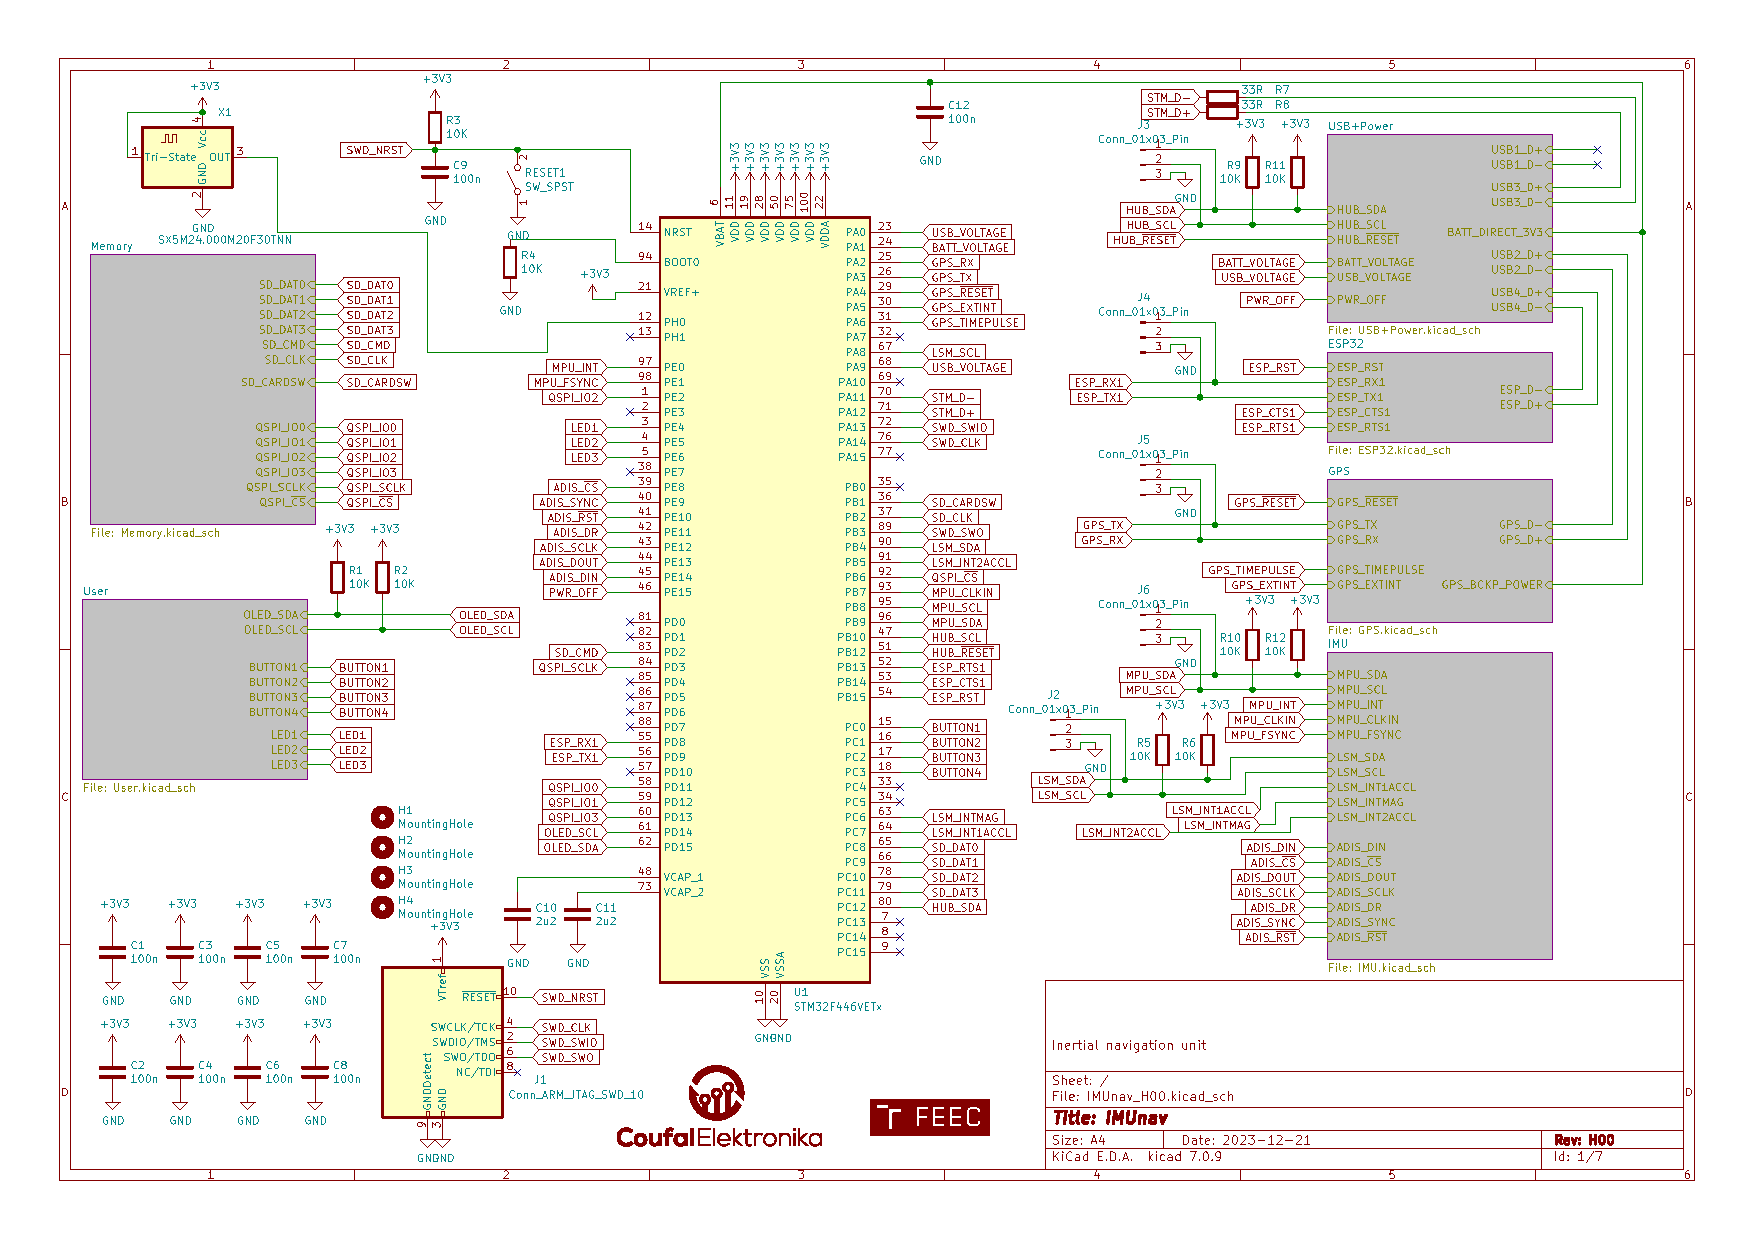
\includegraphics[angle=90, page=1, width=\textwidth]{KiCad/schematic.pdf}

\includegraphics[angle=90, page=2, width=\textwidth]{KiCad/schematic.pdf}

\includegraphics[angle=90, page=3, width=\textwidth]{KiCad/schematic.pdf}

\includegraphics[angle=90, page=4, width=\textwidth]{KiCad/schematic.pdf}

\includegraphics[angle=90, page=5, width=\textwidth]{KiCad/schematic.pdf}

\includegraphics[angle=90, page=6, width=\textwidth]{KiCad/schematic.pdf}

\includegraphics[angle=90, page=7, width=\textwidth]{KiCad/schematic.pdf}

\chapter{Výkres DPS}
\section{Pohled osazení součástek} \label{placementApp}
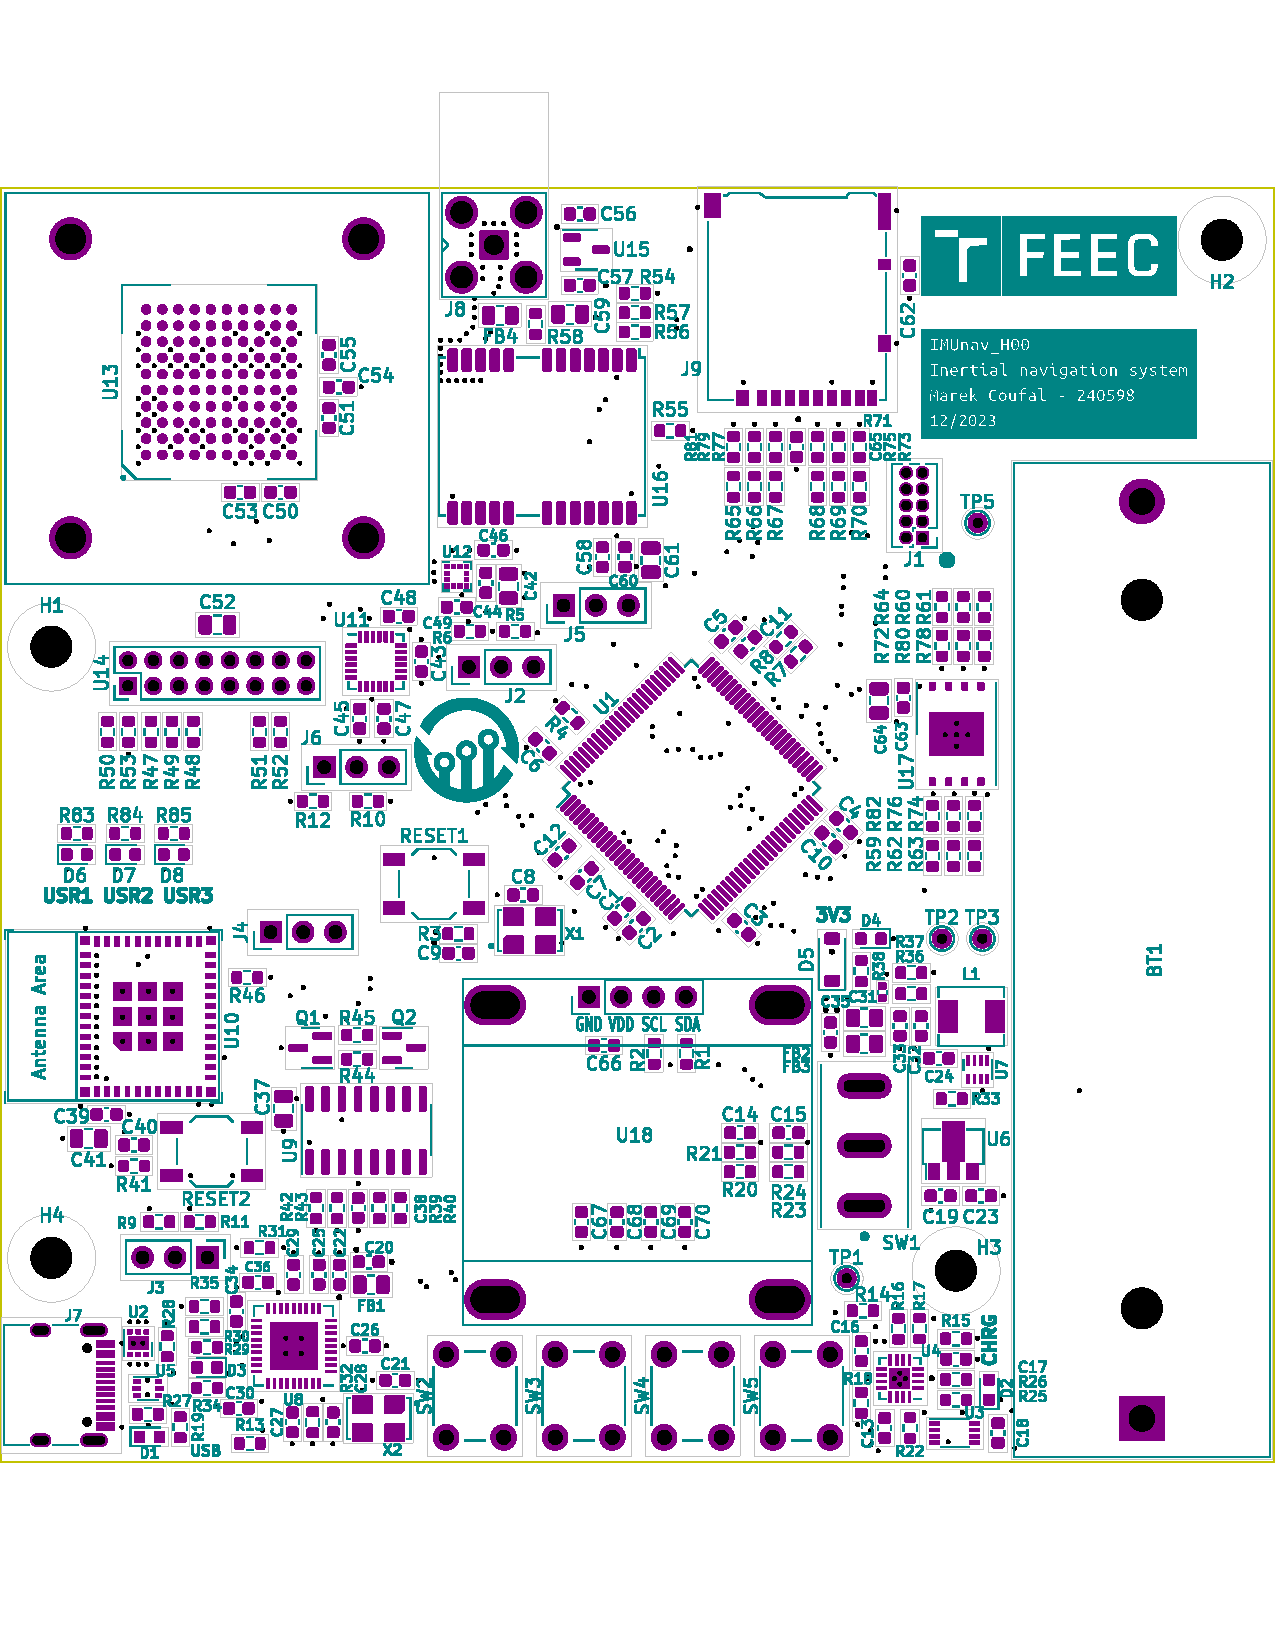
\includegraphics[width=\textwidth]{KiCad/boardTopParts}

\section{Vrchní vrstva mědi DPS} \label{TopApp}
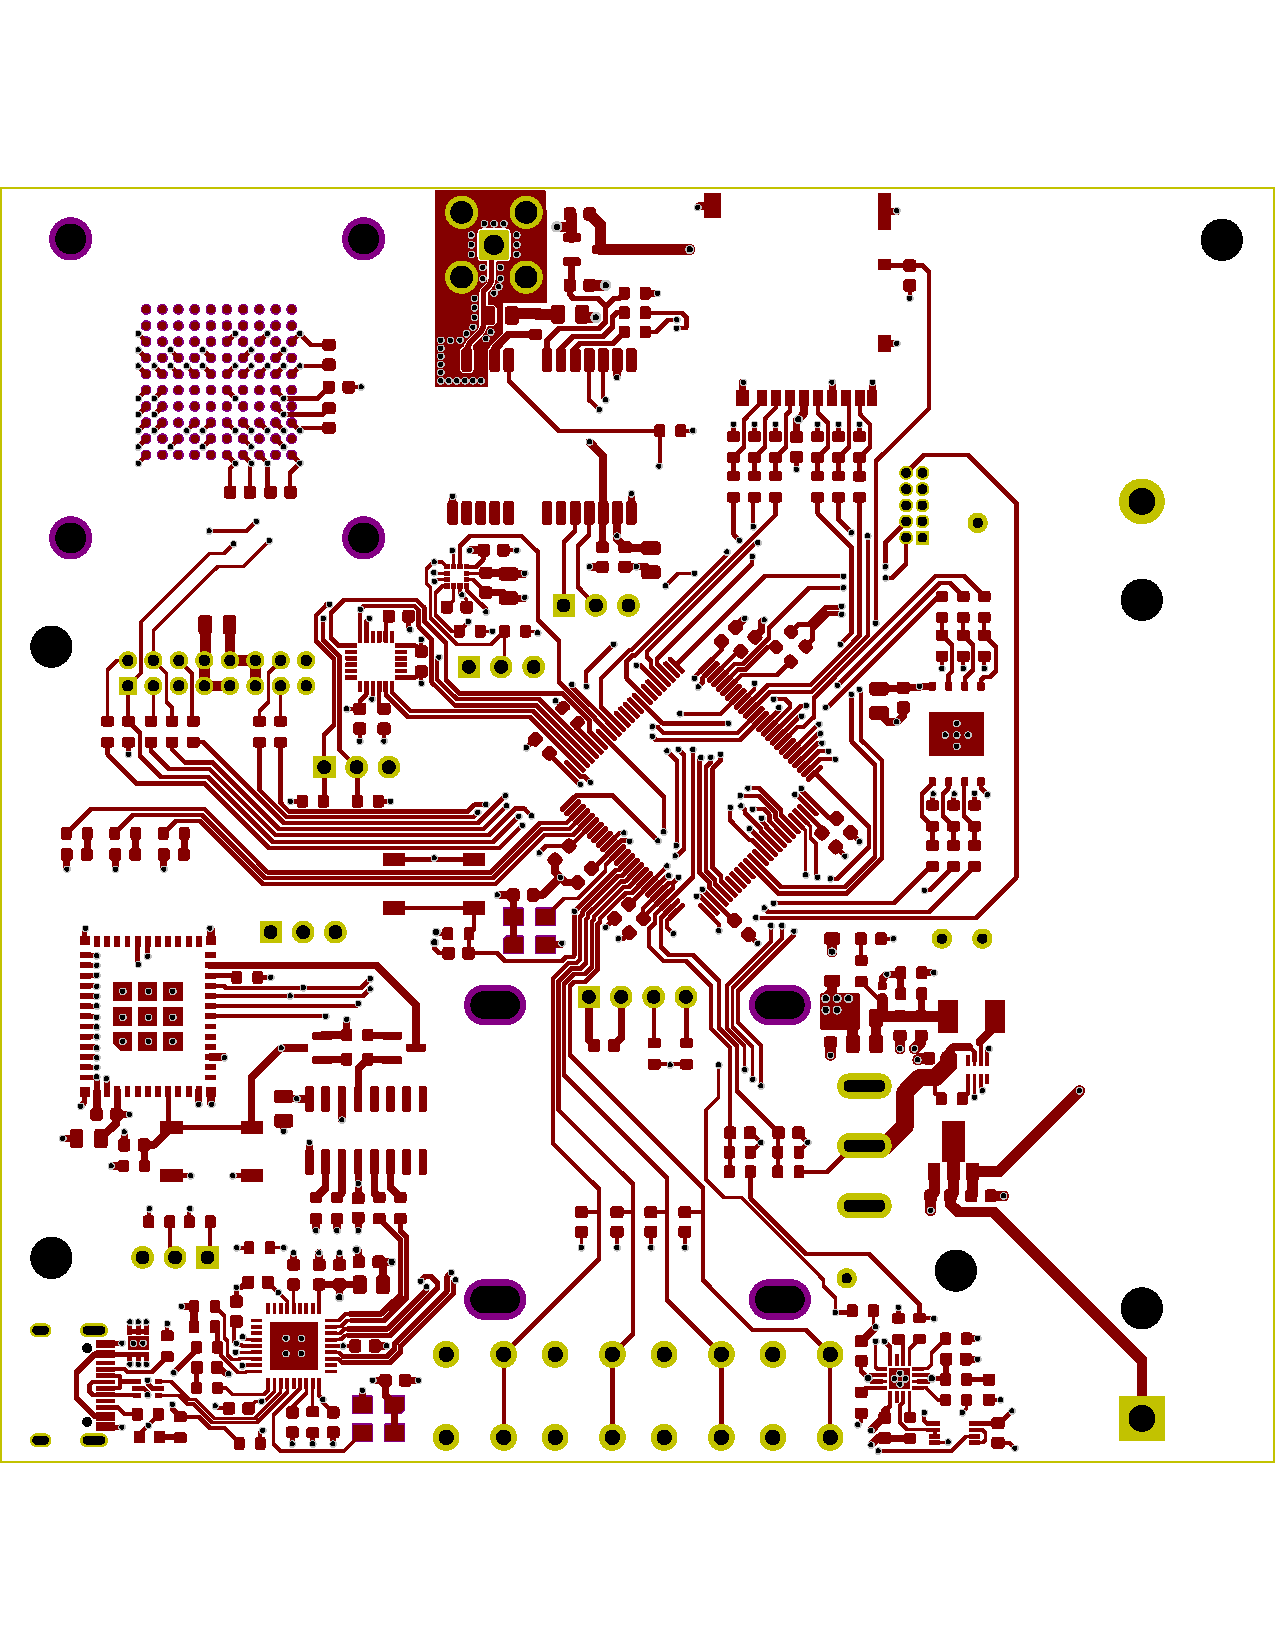
\includegraphics[width=\textwidth]{KiCad/boardF}

\section{Vnitřní vrstva mědi DPS In1}
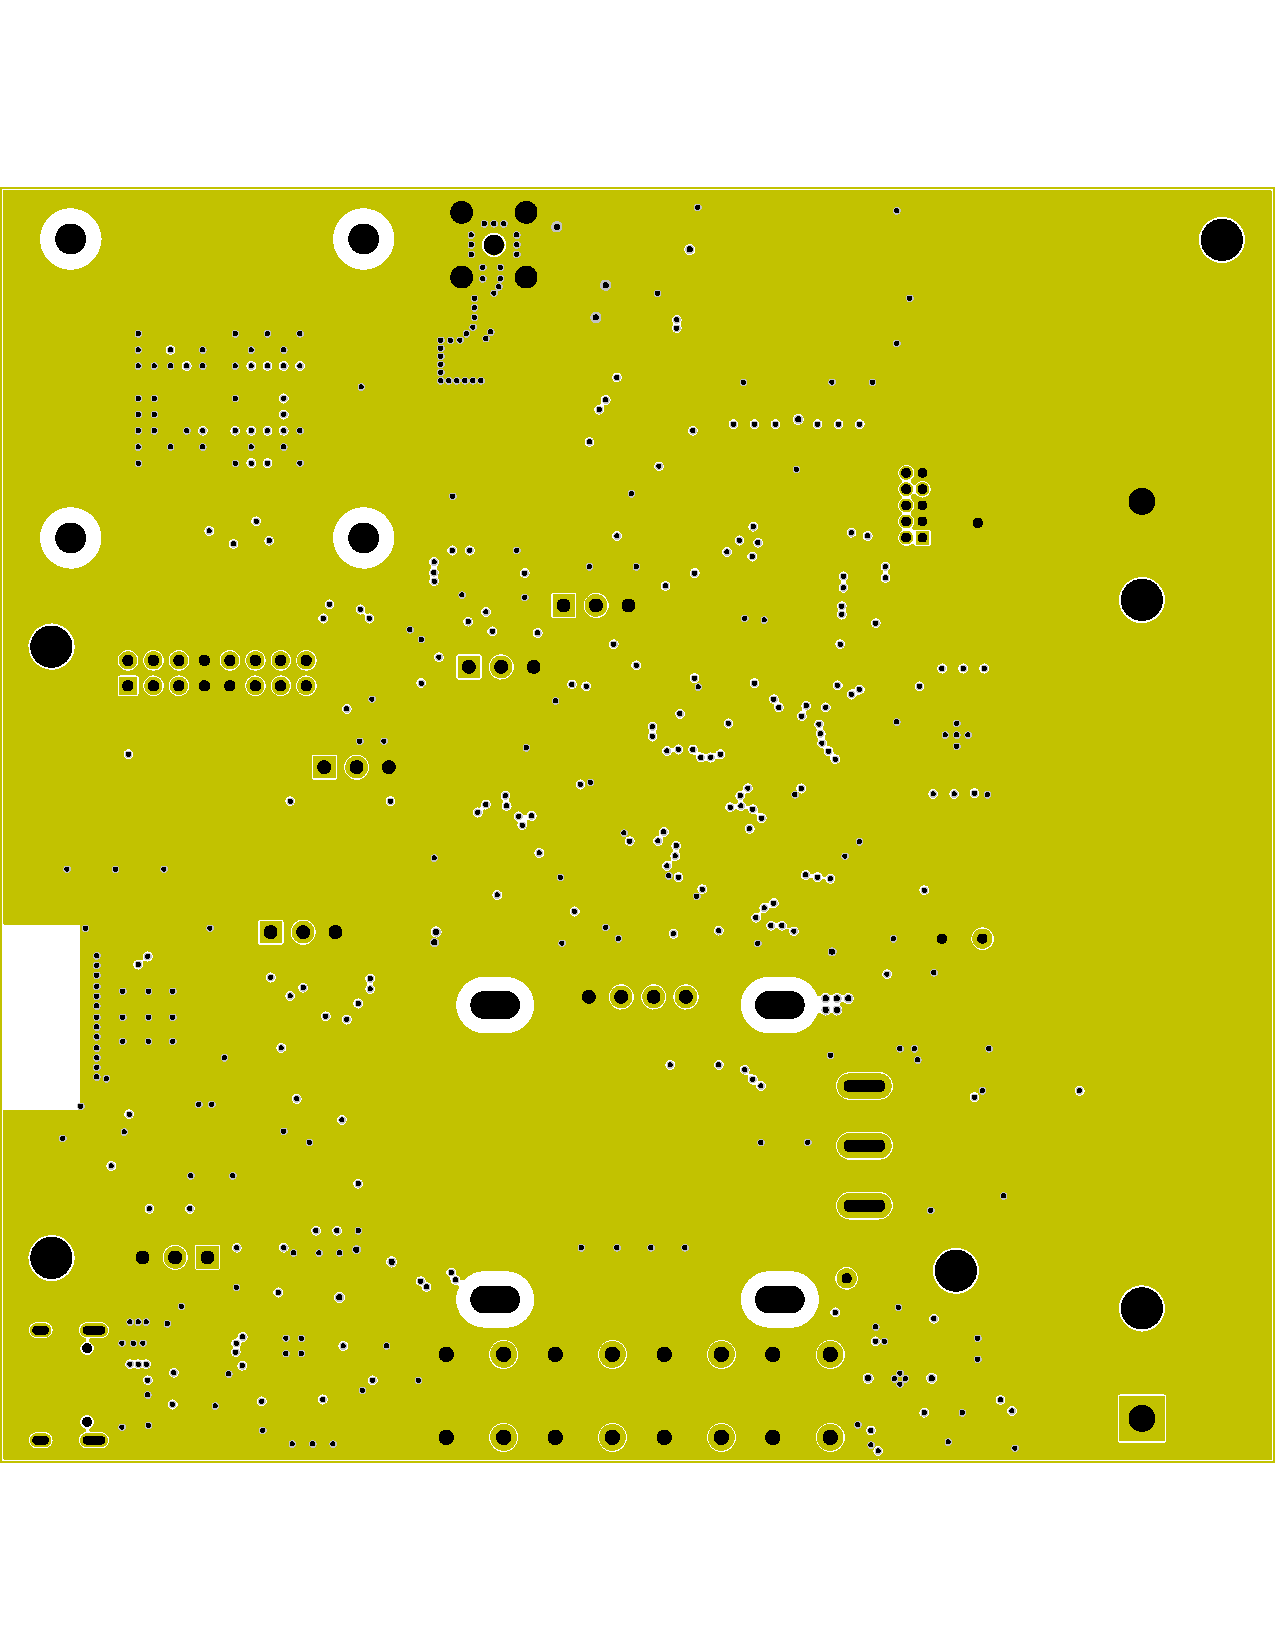
\includegraphics[width=\textwidth]{KiCad/boardIn1}

\section{Vnitřní vrstva mědi DPS In2}
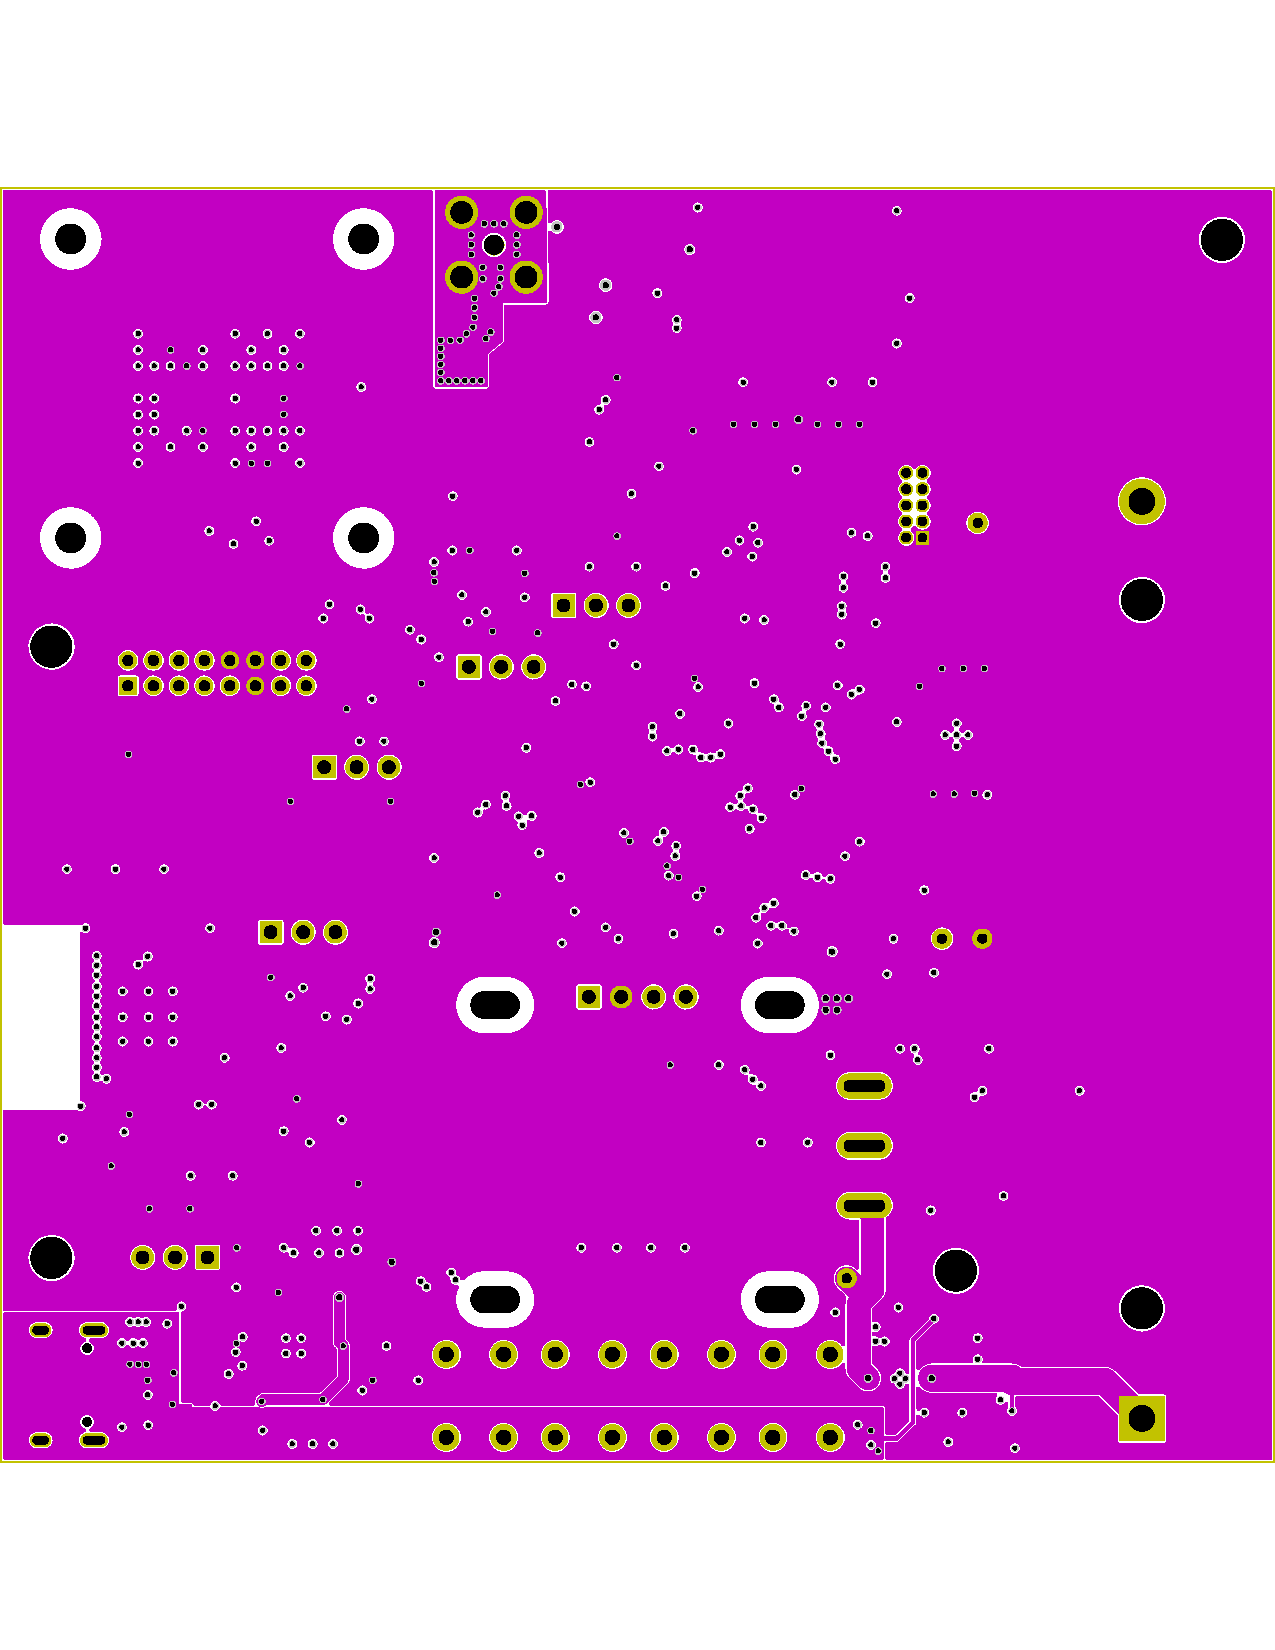
\includegraphics[width=\textwidth]{KiCad/boardIn2}

\section{Spodní vrstva mědi DPS} \label{BottomApp}
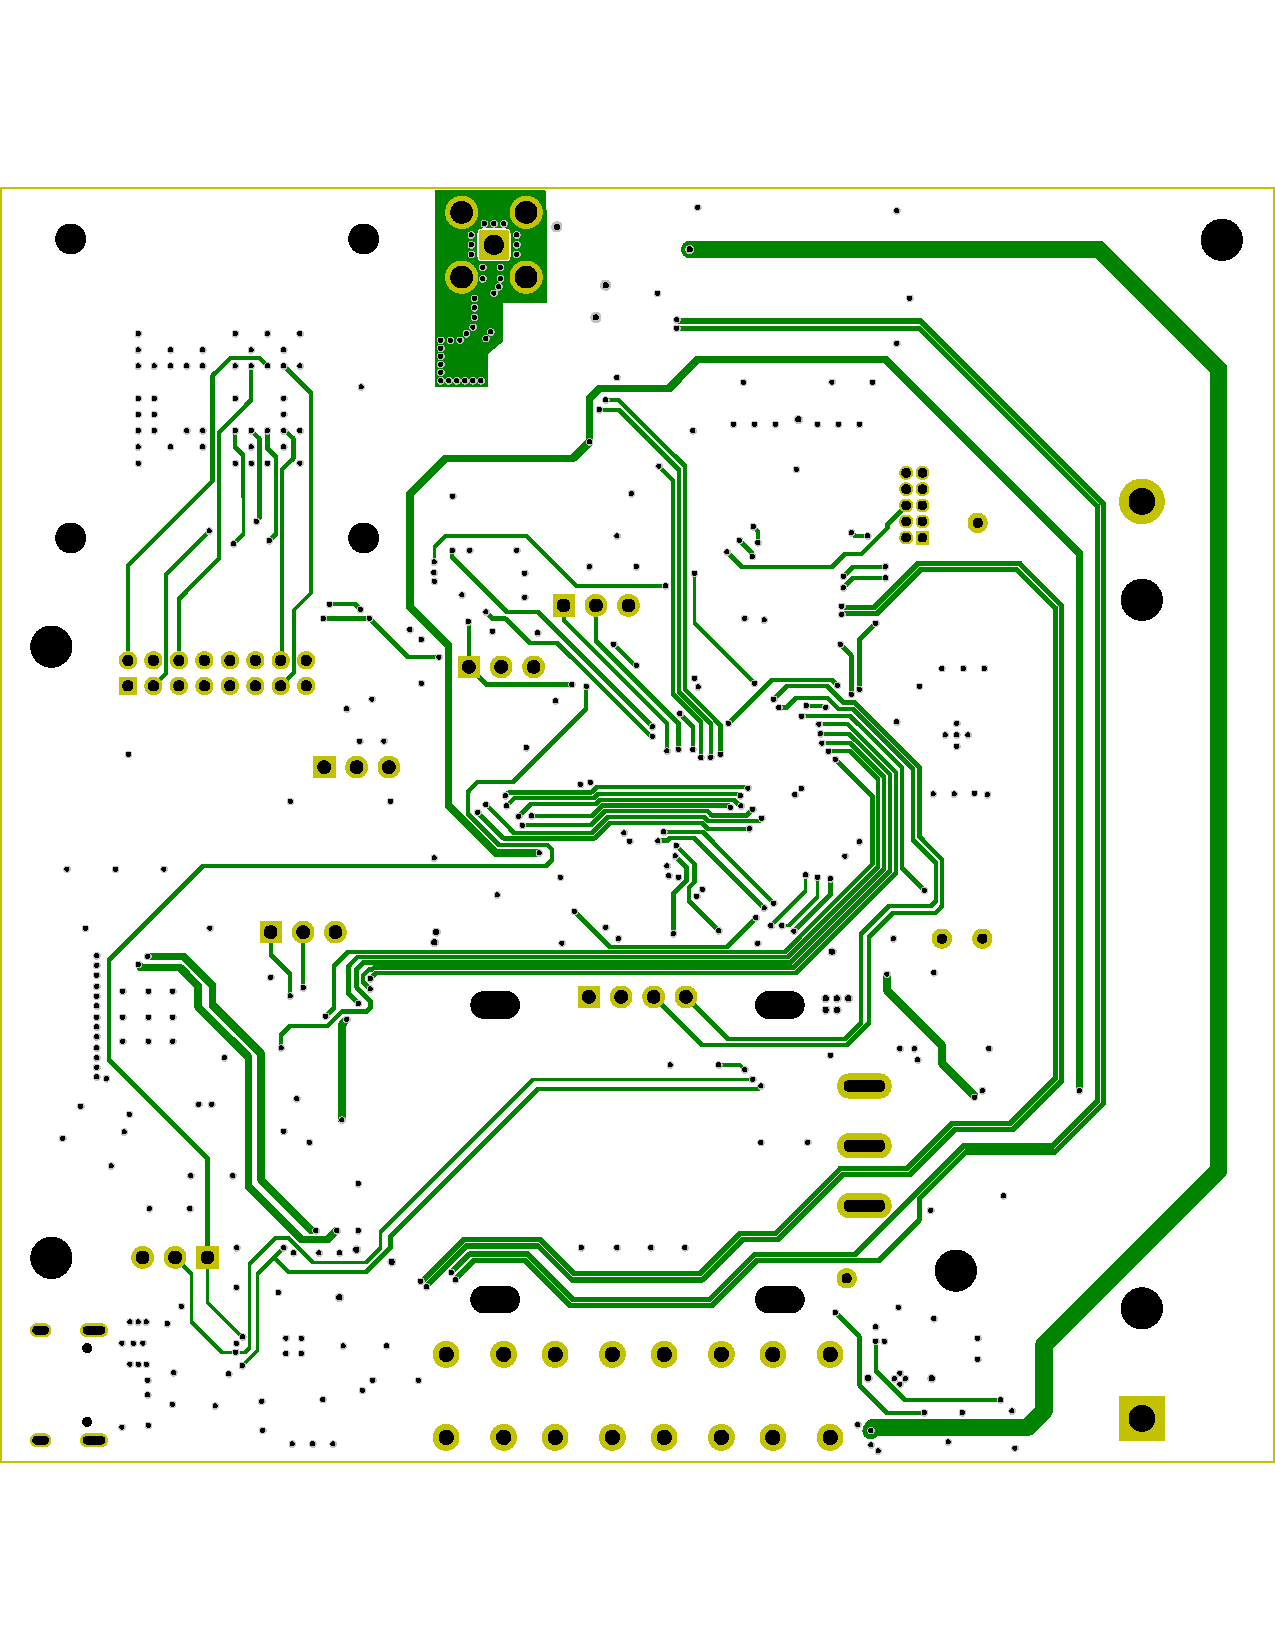
\includegraphics[width=\textwidth]{KiCad/boardB}




\end{document}